% senior_thesis-proposal.tex
% Gregory M. Kapfhammer
% CMPSC 580, Spring 2013
%
% Revised by R. Roos
% Sep 2013
%
% This document provides a sample senior thesis proposal template for use
% by students in Allegheny's CS and Applied Computing programs.
%
%   *******************************************************************
%   * LOOK FOR BLOCK COMMENTS SUCH AS THIS ONE FOR AN EXPLANATION OF  *
%   * THIS DOCUMENT AND HOW TO MODIFY IT FOR YOUR OWN PROPOSAL!       *
%   *                                                                 *
%   * ANY LINE BEGINNING WITH A "%" IS A LATEX COMMENT AND IS IGNORED *
%   * BY THE LATEX PROCESSOR. YOU ARE ENCOURAGED TO COMMENT YOUR OWN  *
%   * LATEX CODE.                                                     *
%   *******************************************************************

%   ********************************************************************
%   * THE FIRST SECTION OF THE LATEX FILE IS THE "PREAMBLE." IT        *
%   * INSTRUCTS LATEX TO IMPORT SPECIAL PACKAGES FOR THINGS LIKE       *
%   * INCLUDING FIGURES, DOUBLE-SPACING, COLORED TEXT, ETC.            *
%   * DEPENDING ON YOUR NEEDS, YOU MAY FIND IT NECESSARY TO USE PACK-  *
%   * AGES THAT ARE NOT INCLUDED IN THIS TEMPLATE. SIMPLY IMITATE THE  *
%   * "\usepackage{...}" COMMANDS SHOWN BELOW.                         *
%   ********************************************************************

%   ********************************************************************
%   * BEGINNING OF PREAMBLE:                                           *
%   ********************************************************************
\documentclass[11pt]{article}

\usepackage[T1]{fontenc}
\usepackage{mathptmx}
\usepackage{amstext}
\usepackage{array}
\topmargin 0.0in
\setlength{\textwidth} {420pt}
\setlength{\textheight} {620pt} 
\setlength{\oddsidemargin} {20pt}
\setlength{\marginparwidth} {72in}

%   ********************************************************************
%   * Many of the commands below were simply copied over from an older *
%   * version of the proposal template; you can just leave them as     *
%   * they are (or you can delve into the TeX/LaTeX documentation      *
%   * and figure out what they do). Otherwise, jump ahead to the next  *
%   * block of comments, where you will enter title, abstract, etc.    *
%   ********************************************************************

\usepackage{fancyhdr} 
\usepackage{url}
\usepackage{graphicx}
\usepackage{color,listings}
\usepackage{calc,xcolor}
\lstset{language=java}
\lstset{breaklines=true}
\lstset{showstringspaces=false}
\lstset{tabsize=3}
\lstset{basicstyle=\ttfamily\scriptsize}
\lstset{breakautoindent=true}
\lstset{postbreak=\space}

% set it so that subsubsections have numbers and they
% are displayed in the TOC (maybe hard to read, might want to disable)

\setcounter{secnumdepth}{3}
\setcounter{tocdepth}{3}

% define widow protection

\def\widow#1{\vskip #1\vbadness10000\penalty-200\vskip-#1}

\clubpenalty=10000  % Don't allow orphans
\widowpenalty=10000 % Don't allow widows

% this should give me the ability to use some math symbols that 
% were available by default in standard latex (i.e. \Box)

\usepackage{latexsym}

% define a little section heading that doesn't go with any number\node [input, name=input] {};
\def\littlesection#1{
\widow{2cm}
\vskip 0.5cm
\noindent{\bf #1}
\vskip 0.0001cm 
}

\pagestyle{fancyplain}

\newcommand{\tstamp}{\today}   
\renewcommand{\sectionmark}[1]{\markright{#1}}
\lhead[\Section \thesection]            {\fancyplain{}{\rightmark}}
\chead[\fancyplain{}{}]                 {\fancyplain{}{}}
\rhead[\fancyplain{}{\rightmark}]       {\fancyplain{}{\thepage}}
\cfoot[\fancyplain{\thepage}{}]         {\fancyplain{\thepage}{}}

\newlength{\myVSpace}% the height of the box
\setlength{\myVSpace}{1ex}% the default, 
\newcommand\xstrut{\raisebox{-.5\myVSpace}% symmetric behaviour, 
  {\rule{0pt}{\myVSpace}}%
}

% leave things with no spacing extra spacing in the final version of the paper
\renewcommand{\baselinestretch}{1.0}    % must go before the begin of doc

% suppress the use of indentation for a paragraph

\setlength{\parindent}{0.0in}
\setlength{\parskip}{0.1in}

\begin{document}


% handle widows appropriately
\def\widow#1{\vskip #1\vbadness10000\penalty-200\vskip-#1}

% build the title section

\makeatletter

\def\maketitle{%
  %\null
  \thispagestyle{empty}%
  %\vfill
  \begin{center}%\leavevmode
    %\normalfont
    {\Huge \@title\par}%
    %\hrulefill\par
    {\normalsize \@author\par}%
    \vskip .4in
%    {\Large \@date\par}%
  \end{center}%
  %\vfill
  %\null
  %\cleardoublepage

  }

\makeatother

%   ********************************************************************
%   * Here is the first place where you need to begin customizing:     *
%   * Enter you name, the title of your proposal, etc., in the places  *
%   * indicated by the comment "% CHANGE!".                            *
%   ********************************************************************

\vspace*{-1.1in}
\title{An Eclipse-based Integrated and Automated Fault Localization System}

% build the author section
\author{
        Tristan Challener\\  % CHANGE!
        Department of Computer Science\\
        Allegheny College \\
        {\tt challenert@allegheny.edu}  \\  % CHANGE!
        \vspace*{.1in} \today \\ \vspace*{.1in}
}

\maketitle       % use the default title stuff

% Default "abstract" environment is too small; customize one instead:
\begin{center}
\large\bf Abstract
\vspace{-1em}  % Reduce space between header and the abstract
\end{center}

%   ********************************************************************
%   * Here is the second place where you need to customize:            *
%   * enter your abstract in the "quote" environment:                 *
%   ********************************************************************

\begin{quote}
  
	We propose the implementation and evaluation of an Eclipse plugin to
	display per-test coverage information and risk evaluation.  This
	research and implementation project will involve several phases.  In
	the first phase, we will investigate the relative effectiveness of
	several risk evaluation functions.  We will empirically evaluate 
	multiple theoretically effective functions based to determine the 
	most practical choice to include in our final plugin.  The next phase
	will involve the use of the CodeCover system to generate per-test 
	coverage information for several test systems.  In the third phase of
	the project, we will implement a system to utilize CodeCover coverage
	output to display per-test coverage information inside Eclipse, and will
	perform risk evaluation using the above chosen technique.  Finally, we
	will evaluate the system using a human study involving programs 
	with faults introduced by the MAJOR mutation framework.  The results 
	of the study will include deeper understanding of the value of per-test 
	coverage and suspiciousness ranking as tools for fault localization. 

\end{quote}

%\vspace*{-.4in}
\section{Introduction}
\label{sec:introduction}
\vspace*{-.1in}

%   ********************************************************************
%   * Enter the text of your introductory section here.                *
%   ********************************************************************

The process of debugging can be complex and difficult.  The first task
associated with debugging is identifying the fault, and this step,
\emph{fault localization}, is the most expensive in terms of time cost
\cite{harrold}. At present, the process of fault localization is mostly
manual, though several techniques exist that attempt to automate the
process.  A number of these techniques are described in detail below.
Many of these automated fault localization techniques (AFLs) compare the
flow of execution through a faulty program when executing passed and
failed test cases.  This type of approach employs \emph{coverage
monitoring}, the tracking of which statements are executed by test
cases.  Any statement that is executed is said to be \emph{covered}.
Tools such as Java Code Coverage (JaCoCo) \cite{jacoco} provide
information regarding which statements are covered by a supplied test
suite.  By analyzing code coverage for different test cases, these AFLs
seek to determine which statements are most likely to contain the fault.

Many Coverage tools exist, including those designed for integrated development
environments such as Eclipse.  For example, JaCoCo provides interactive
coverage monitoring within Eclipse.  However, JaCoCo only reports total
coverage for a test suite; that is, the tool reports which statements
were covered, partially covered, or not covered after execution of all
of the test cases.  This system does not report on coverage of
individual test cases.  Since \emph{per-test coverage} is vital to the
application of several fault localization techniques, the lack of such
information leads to increased difficulty in applying those techniques.

As an alternative to the more popular JaCoCo, we will make use of a
lesser known tool called CodeCover.  Though a number of interfaces are
provided, including command-line and Apache Ant, we will focus on the
Eclipse plugin for the purpose of this project.  Unlike JaCoCo,
CodeCover is designed to produce coverage on a per-test basis.  The
system includes support for breaking coverage information for a JUnit 
test suite or test case for each test method, automatically generating
a distinct coverage report for each test method.  This functionality
makes CodeCover ideal to the goals of this project.

The purpose of this research project is to develop an Eclipse plugin
which displays the per-test coverage from a test suite and per-statement
suspiciousness analysis, through an interactive system, as well as to
demonstrate its effectiveness.  The plugin will allow a programmer to
select individual or multiple test cases and view their coverage.  We
hypothesize that making per-test coverage, the basis for many fault
localization techniques, readily available will allow programmers to
more rapidly identify faults in programs.  This hypothesis will be
investigated through human study, employing experienced programmers,
specifically undergraduate students, to compare
the benefits of per-test coverage when compared to full suite coverage.
To generate test cases for evaluating our plugin, we will introduce
faults into programs using the MAJOR mutation analysis system
\cite{major}.

\vspace*{-.1in}
\section{Related Work}
\label{sec:relatedwork}
\vspace*{-.1in}

\subsection{Automated Fault Localization Techniques}

There are a wide variety of existing fault localization techniques
\cite{harrold}. Many of these methods make use of per-test coverage
analysis, such as Set-union, Set-intersection, Nearest Neighbor, and
Tarantula.  There are other AFLs that do not use per-test coverage, such
as Cause Transitions \cite{cause}, but they are outside the scope of this project.  

Set-union and Set-intersection compare the coverage of a single failed
test case to the coverage of all of the passed test cases.  Set-union
defines the initial set of suspicious statements by the set of all test
cases visited by the failed test case but not visited by any passed test
cases.  Conversely, Set-intersection defines the initial set as the set
of all statements visited by every passed case but not by the failed
test case.  Nearest Neighbor works similarly to the previous techniques,
but instead of considering all of the passed test cases, it only
considers one.  By some method, the passed test cases that is most
similar to the failed test case is identified.  Nearest Neighbor defines
the initial set as the set of all statements visited by the failed case
and not by the passed case.

Tarantula is notably different from the previously mentioned techniques.
Instead of determining a set of suspicious statements, Tarantula ranks
techniques in order of suspiciousness.  However, Tarantula still
utilizes per-test coverage reporting.  In their paper, Jones and Harrold
present an empirical analysis which indicates the superiority of
Tarantula in both efficiency and effectiveness when compared to the
other techniques described above, as shown in Figure 1 \cite{harrold}.  Since Tarantula
uses per-test coverage, this provides substantial evidence for the
importance of per-test coverage in the fault localization process.

\begin{figure}
  \centering
  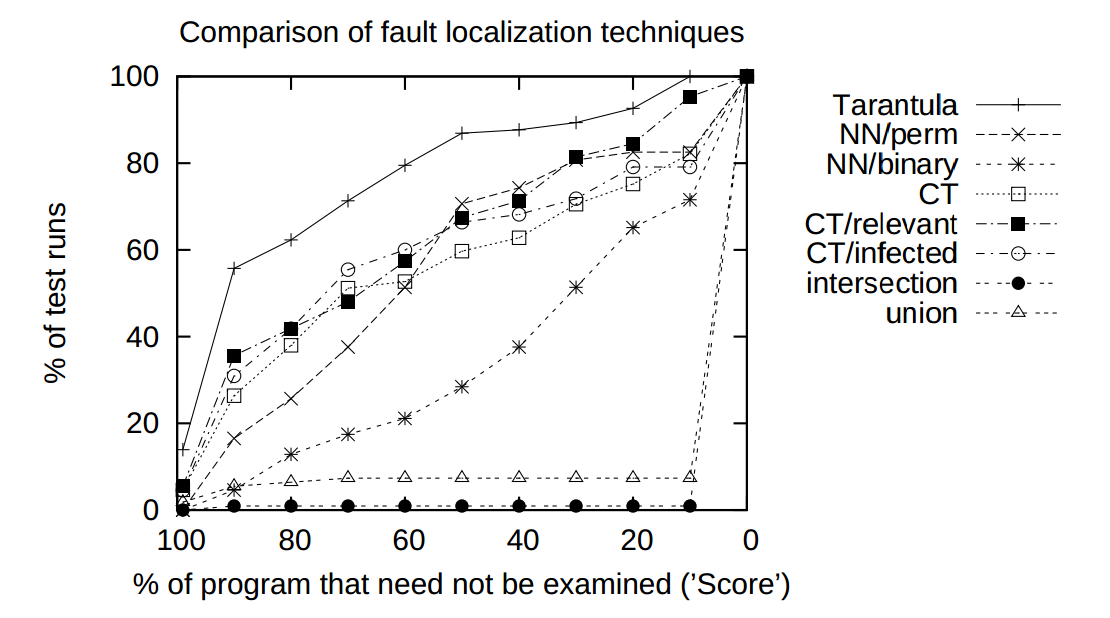
\includegraphics[width=0.9\linewidth]{img/tareff.png}
  \caption{An empirical comparison of several fault localization
  techniques by percentage of code eliminated from consideration.  The
  graph plots percentage eliminated (determined by the rank of the
  faulty statement) against frequency that the tool achieved that level
  of success.  Tarantula is demonstrated to achieve better results more
  often than other techniques.}
  \label{tareval}
\end{figure}

Xie et al. present an alternative discussion of various risk evaluation 
functions focusing primarily on theoretical correctness \cite{theory}. They 
argue that many existing risk evaluation formulas are actually functionally
equivalent.  In addition, they provide theoretical analysis that shows the 
superiority of specific functions relative to one another both within 
functionally equivalent groups and between those groups. Through detailed
theoretical proof they show that the equivalent sets ER1 and ER5 are maximal
for accurately calculating suspiciousness.  The ER1 set includes a pair of 
formulas studied in a paper by Naish et al. \cite{naish}  The ER5 equivalent 
set includes three functions, two of which are also studied in the paper
by Naish et al. The third is discussed in a paper by Wong et al. \cite{wong}
It is important to note that all the above risk evaluations also require
per-test coverage data.

As a followup to the paper by Xie et al. mentioned above, Qi et al. \hspace*{-0.7mm}\cite{genprog}
performed a detailed empirical to study the practical effectiveness of the 
theoretically maximal functions as proven by Xi et al.  This study includes
a wide variety of risk evaluation functions, and compares them by applying 
them to practical, real-world programs and faults.  The various formulas
were inserting them into popular automated program repair system GenProg.
GenProg uses genetic programming, applying a risk evaluation function to 
repeatedly alter a faulty program by mutating suspicious statements.  In their
study, Qi et al. \hspace*{-0.5mm}modified GenProg to use several different formulas.  By 
comparing the effectiveness of automated repair when using each different 
risk evaluation function, they were able to provide substantial empirical
evidence regarding the superiority of certain formulas.  Note that this method
of comparison differs from that pursued by Jones and Harrold \cite{harrold}, 
discussed previously, which compared the relative suspiciousness ranking of 
faulty statements (referred to as EXAM score).

Surprisingly, Qi et al. did not confirm the results shown by Xie et al.
Instead, they found that several functions, eliminated from consideration
as maximal functions early in the proof provided by Xie et al., were actually better than expected. Specifically,
Qi et al. show that in practice, the Jaccard risk evaluation function performed
equally as well or better than all other formulas considered.  They conclude that,
at least within the context of automated program repair, Jaccard should be 
favored when choosing a risk evaluation function.  In addition, they further 
conclude that the EXAM score method of comparing these formulas does not 
accurately reflect their relative performance in the context of automated
program repair.

In another paper \cite{parnin}, Parnin and Orso performed a human study about the
real-world effectiveness of fault localization techniques.  In that
study, they asked participants, graduate students in computer science
with varying levels of experience, to perform debugging tasks.
Participants were asked to compare their experiences when using standard
debugging practices with using an Eclipse plugin designed to display
Tarantula suspiciousness ranking.  The authors also considered the
relative average amount of time required for each task, with and without
the plugin.  

As part of their results, Parnin and Orso concluded that
although exact ranking of suspicious statements does not often directly
lead to localization of the fault, it is helpful as a starting point.
We therefore hypothesize that the per-test coverage information used to
obtain suspiciousness ranking will itself provide substantial assistance
in fault localization.

\subsection{CodeCover Coverage Analysis}
CodeCover produces coverage information for Java, and has built in 
functionality for generating coverage information on a per-test suite,
per-test case, and even per-test method basis.  In addition, CodeCover
is designed to function within Eclipse.  All parts of the coverage
monitoring process can be done through the Eclipse development
environment.  Since the final goal of this project is to produce an
integrated Eclipse tool for fault localization, using per test
coverage and risk evaluation, CodeCover is ideally suited to our
purposes.  

\begin{figure}[htpb]
  \centering
  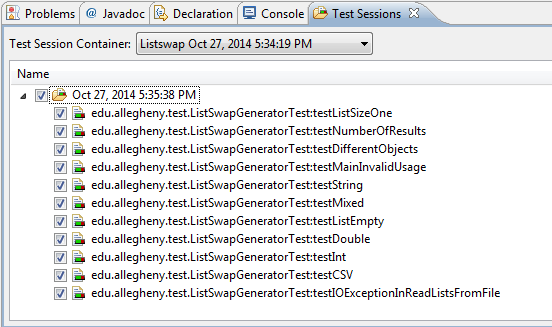
\includegraphics[width=4in]{img/codecoverpertest.png}
  \caption{Screenshot of CodeCover Eclipse plugin displaying per-test coverage
  output from a single execution of a JUnit test suite.}
  \label{codecover}
\end{figure}

CodeCover works in several stages.  The first step to acquiring coverage
information is instrumentation.  During instrumentation, numerous
statements are procedurally inserted into the Java source files which 
are to be included in the coverage analysis.  In the context of Eclipse,
these files are manually marked, since there may be source files for 
which coverage information is unnecessary.  The statements that are 
inserted during instrumentation record various information as the code
is executed, including which existing Java statements were executed, and
which test case or method exeucted them.  After instrumentation is
complete, the newly instrumented source files, as well as any other source
files, are compiled as normal.

CodeCover provides functionality for using existing JUnit test cases and
test suites for coverage analysis. With an existing Eclipse project with 
a JUnit test class, CodeCover can simply be enabled and executed.  By 
default, CodeCover produces output in the form of a several coverage
reports.  The output includes a full coverage report for every test method 
within the JUnit test; that is, per-test coverage data, as shown in Figure
\ref{codecover}.  

After executing a test process through the CodeCover Eclipse, per-test
coverage can be viewed in several ways.  First, coverage can be viewed on 
a per-test basis within Eclipse.  As shown in Figure \ref{codecoverage}, 
selecting one or more test methods displays coverage information for those
test methods only.  In addition to viewing coverage within Eclipse, CodeCover
allows coverage information to be executed in a variety of formats.  Using
provided template XML (eXtensible Markup Language) files, coverage data can be exported, for example, as
hierarchical HTML (HyperText Markup Language) documents or as CSV (Comma Separated Value) files.  

\begin{figure}[tpb]
  \centering
  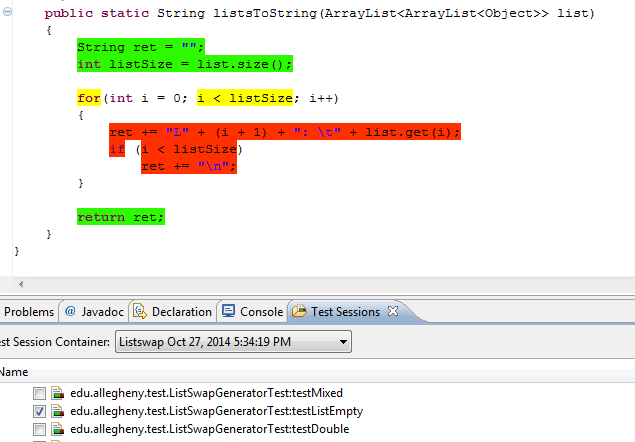
\includegraphics[width=4in]{img/codecovercoverage.png}
  \caption{Screenshot of CodeCover Eclipse plugin displaying coverage
  highlighting for a single test method.  Statements highlighted in green
  were covered by this test method, and those in red were not.}
  \label{codecoverage}
\end{figure}

\subsection{MAJOR Mutation}

MAJOR is a fault seeding and mutation analysis tool that integrates
directly into the Java compiler \cite{major}. \emph{Mutation} is the process of
intentionally introducing faults into a program for various purposes,
including evaluation of test suite quality and testing for fault
localization techniques.  Mutants generated are either \emph{killed} by
the test suite or \emph{live}.  A mutant is killed if a test case fails;
that is, the test suite was sufficient to identify the fault.  Live
mutants either indicate that the test suite is insufficient or that the
introduced fault was in fact logically equivalent to the original code.

MAJOR can perform a number of conditional mutations, including replacing
binary arithmetic, logical, relational, shift and unary operators with
valid alternatives.  Figure 4 shows an example of one
possible mutation performed by MAJOR.  The tool can also replace literal
values with alternatives; these various mutation types can be selected
with compiler operators.  Along with the domain specific language
provided by MAJOR, this allows for great flexibility and extensibility.
Additionally, MAJOR has been shown to be relatively efficient, with only
about 15\% runtime overhead.  It is also noteworthy that MAJOR utilizes
coverage analysis to improve efficiency.

A technical report by Just et al. \cite{mutants} indicates a statistical
correlation between mutant detection and real world fault detection.
Although they also note that as much as 20\% of real world faults cannot
be represented by mutants, this still suggests that mutants are a viable
substitute for real world faults in the context of software testing and,
similarly, fault localization.

\begin{figure}[tbp]
  \centering
  \begin{lstlisting}
public static Type classify(int a, int b, int c) {
		int trian;
		if (a <= 0 || b <= 0 || c <= 0)
			return Type.INVALID;
		trian = 0;
	        ... (additional statements) ...
}
\end{lstlisting}

  \begin{lstlisting}
public static Type classify(int a, int b, int c) {
		int trian;
		if ((a <= 0 || b <= 0) != c <= 0)
			return Type.INVALID;
		trian = 0;
	        ... (additional statements) ...
}
\end{lstlisting}

  \caption{(top) Original program and (bottom) program after mutation.}
  \label{majorex}
\end{figure}

\vspace*{-.2in}
\section{Method of Approach}
\label{sec:method}
\vspace*{-.1in}

The first phase of this project will involve an empirical study of
risk evaluation functions to determine what would be the optimal
choice to integrate into our final Eclipse-based system.  Using the
results of previous studies we will select a set of candidate formulas.  
These will include the theoretically optimal functions \cite{theory} 
and those functions shown to perform better in practice using multiple 
comparison techniques \cite{harrold, genprog}.  The list of risk evaluation 
functions in Table \ref{riskeval} shows some functions which will be considered.
This list is not complete, and is subject to change; it is included only
as a example, and is not to be taken as complete or final.

\begin{table}
	\centering
	\begin{tabular}{|l| >{$} c <{$} |}
	\hline
	Naish         & a_{ef} - \frac{a_{ep}}{a_{ep} + a_{np} + 1}\\\hline
	Russel \& Rao & \frac{a_{ef}}{a_{ef} + a_{nf} + a_{ep} + a_{np}}\\\hline
	Tarantula     & \frac{a_{ef}}{a_{ef} + a_{nf}} / \left( \frac{a_{ef}}{a_{ef} + a_{nf}} + \frac{a_{ep}}{a_{ep} + a_{np}} \right)\\\hline
	\end{tabular}
	\caption{Some risk evaluation techniques shown to be effective \cite{harrold, genprog} }
	\label{riskeval}
\end{table}

Our preliminary investigation suggests that using EXAM score to compare 
the functions we choose to study will provide the most relevant comparison 
of the formulas within the context of our goals.  Since we are not performing
automated programming repair, and are instead using the risk evaluation
function to direct manual debugging, it makes more practical sense
to evaluate the functions based on their success rate in ranking faulty
statements high in the list of suspiciousness.

For this empirical study, our subject programs will be drawn from the 
Siemens suite avalible within the Software-artifact Infrastructure 
Repository (SIR) \cite{sir}.  We will choose only artifacts which include
JUnit test suites, since the Eclipse plugin we develop will 
utilize per-test coverage generated from JUnit tests.  As mentioned above,
we will input the per-test coverage generated by CodeCover into a selected
set of risk evaluation functions, and calculate their EXAM score.  Note
that EXAM score, mentioned in Section \ref{sec:relatedwork}, evaluates risk evaluation
functions by the relative rank of the faulty statement within the result
set of suspicious statements.  This value indicates the percentage of
statements that must be need not be examined, as seen in Figure \ref{tareval},
and is a higher-is-better metric.

Optimally, we will find a single risk evaluation function that consistently
proves to have a statistically significant high EXAM score relate to 
other formulas.  Should this be the case, we will select this risk evaluation
function to use exclusively for fault localization within our Eclipse
plugin.  If multiple risk evaluations prove to have similar success, we
will instead arbitrarily choose a default function and allow the user to
select one of the others within the Eclipse plugin (as well as change the
default behavior).

The Eclipse integrated development environment will be used to display
per-test coverage information.  We will design a plugin for Eclipse
which will highlight statements executed by a given test case, similarly
to the behavior of the CodeCover Eclipse plugin described in Section \ref{sec:relatedwork}.  Upon first
execution after changes are made to a program, the plugin will request updated
coverage information from the CodeCover plugin.  Once the coverage analysis
is complete, we will extract the relevant information from the XML test
container produced by CodeCover.  Our plugin will parse this output using a
DOM (Document Object Model) approach, storing the XML document inside a Java
program as a Tree structure.  Once parsing is complete, it will perform another
pass of the DOM in order to determine which statement node corresponds to each
line of code in the source, and from there which test case covered each of these
statements.

After our plugin has extracted the necessary information from CodeCover's
output, it will build a simplified representation of the coverage information
to allow easy application of selected risk evaluation functions.  This 
simplified format will be as indicated in Table \ref{riskeval} (for each 
statement, store $a_{ef}, a_{ep}, a_{nf}, a_{np}$), since for risk evaluation
we do not need information regarding which tests executed a given statement,
only the number of tests which did so.  We will apply the single selected
risk evaluation function, and organize the output as an ordered list of
statements according to suspiciousness.  

We will provide a number of features to users within our Eclipse plugin.
First, we will allow users to select single test methods and view the 
coverage information linked to that test.  Similarly to CodeCover, shown in
Figure \ref{codecoverage}, we will highlight covered statements in green
and uncovered statements in red.  We will also clearly indicate, in the list
of available test methods, which tests passed and which failed.  This will
allow users to investigate failures by showing exactly which tests executed
or did not execute a given statement, in the context of test failure or success.
Finally, we will provide functionality for selecting a single statement and
viewing a list of tests which covered that statement, similar to as shown in
Figure  \ref{tarex}, but without absolute suspiciousness value (and using test
method names).

\begin{figure}[tpb]
  \centering
  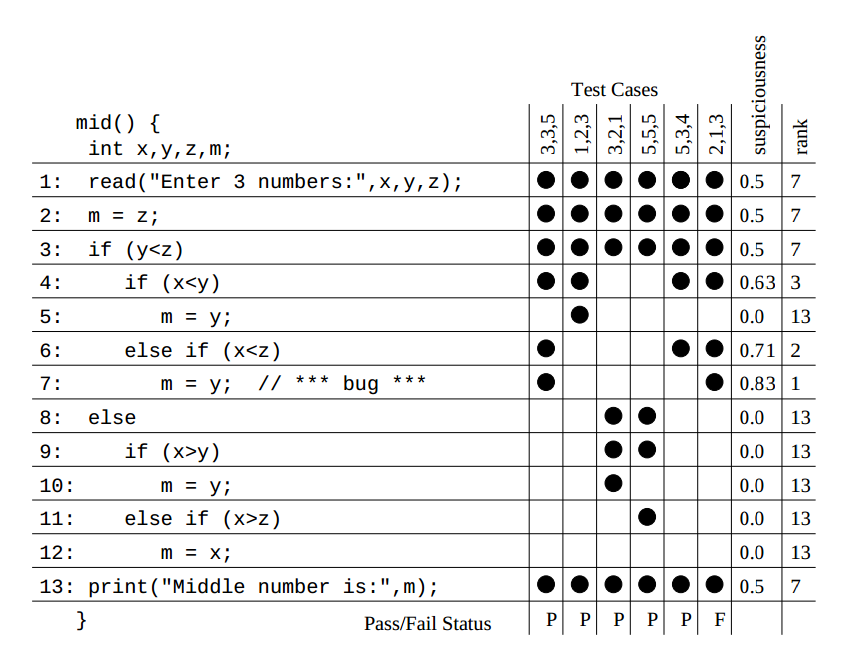
\includegraphics[width=4in]{img/tar.png}
  \caption{An example of the suspiciousness rating and ranking provided
  by Tarantula.  A dot in a column indicates that the associated
  statement was covered by that test.}
  \label{tarex}
\end{figure}

In addition to the coverage view, we will also provide a view for navigating
suspicious statements.  We will provide an ordered list of statements, as links,
from least suspicious to most.  In addition to navigating this way, we will also
provide functionality for highlighting all statements with a single color of
varying opacity, where the opacity of a statement's highlighting is a function
of its suspiciousness.  This will allow users to identify suspicious blocks of code
at glance.  The purpose of this function is to counteract the argument made by 
Parnin and Orso that isolated statements (without context), are not always enough
to locate a fault \cite{parnin}.

\vspace*{-.2in}
\section{Evaluation Strategy}
\label{sec:evaluate}
\vspace*{-.1in}

The evaluation of the plugin will be two-fold: correctness and effectiveness.
First, we will consider correctness.  Our system for parsing exported CSV
files will be thoroughly tested to ensure the coverage data is being
correctly extracted.  Will verify this correctness by manually comparing
the list of tests covering individual statements within the CodeCover plugin
and according to the parsed data.  This will establish confidence that there
was no loss or corruption of data produced by CodeCover.  Furthermore, we 
will design a JUnit test suite for ensuring that our simplified coverage
data representation is built correctly.

Secondly, we will consider the effectiveness of the tool as an
assistance to fault localization in the debugging process.  To that end,
we will perform a human study involving a group of undergraduate
programming students.  In his paper, Tichy notes that studies that use 
students as subjects are still worthwhile, for several reasons \cite{students}.
For example, he notes that students subjects can be helpful at identifying
trends, and are in fact a prerequisite for encouraging professional 
participation in any case.  He argues that experiments must be debugged with 
students prior to running them with professionals.  In addition, student
subjects can be used to eliminate some hypotheses.  As such, we conclude
that the use of undergraduate programming students is valid.

All students will be educated on the use of the
tool prior to using it.  For this study, we will choose two programs of
similar complexity and introduce a fault, as described above.  These two
programs will include an exhaustive test case with at least 95\%
coverage, and the seeded fault will have been killed by the test case
(indicating that the provided test cases are sufficient to identify the
fault).


\begin{figure}[htbp]
  \centering
  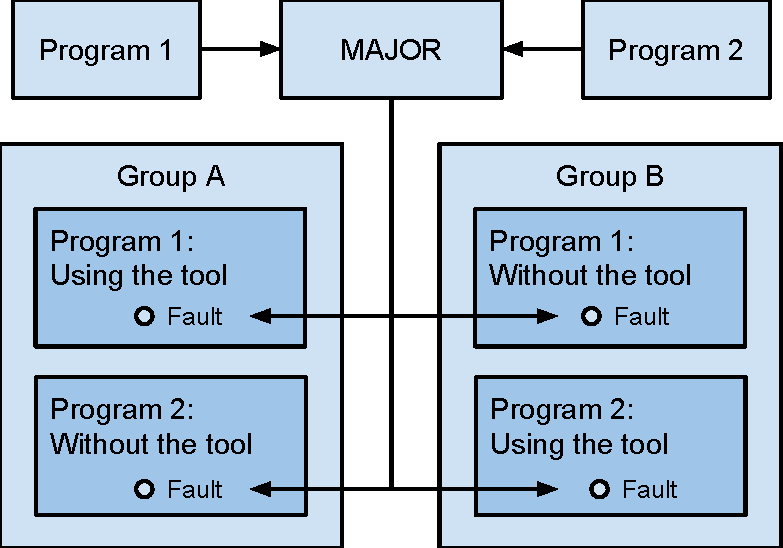
\includegraphics[width=0.65\linewidth]{img/study.pdf}
  \caption{Diagram representing the human study.  MAJOR inserts a fault
  into two programs, and students are assigned to use tool for one
  program and not the other (groups A and B).}
  \label{studyd}
\end{figure}

Since the students will have varying levels of experience (including
different classes or internship experience), they will work
independently.  Each student will be arbitrarily assigned one program to
debug with the tool and one program to debug without the tool (divided
into two groups, as shown in Figure 6).  The
students will have no prior access to either program, to allow fair
analysis of their experience.  For each student, their time to identify
each fault will be recorded.  Up to thirty minutes will be allowed for
each program; after that time has expired, the student will be asked to
stop their debugging process and continue to the next task.  

Evaluation of effectiveness will involve a comparison of each the
average completion times for each debugging task with the tool and
without the tool.  If the tool is effective, students will, on average,
complete a task notably faster when using the tool.  In addition,
students will complete the task more often when they have access to the
per-test coverage tool.

Aside from completion time, we will also ask involved students to
complete a detailed survey after they have finished with both tasks.
This survey will include questions relating to the manner in which the
tool was used, and how helpful the tool was in completing the problem.
Specifically, we will ask students to reflect on the component of the
tool which was most useful in solving the problem (i.e., suspiciousness
ranking, suspiciousness rating, per-test coverage highlighting, or
per-statement test listing).  Students will also be asked to comment on
their level of experience with Java, and describe their familiarity with
the programs used for analysis.  Evaluation of the effectiveness of the
tool will account for comments made by students in this survey.  For
example, if a student reports that he was already highly familiar with
the code, their completion times may be less valuable than those of
students with limited exposure to the code.

\vspace*{-.1in}
\section{Research Schedule}
\label{sec:schedule}
\vspace*{-.1in}

\subsection{Thesis Outline}
The final thesis paper for this project will consist of six chapters, 
as follows:
\begin{enumerate}
\item Introduction
\item Related Work
\item Method of Approach
\item Results: Empirical Study
\item Results: Human Trial
\item Conclusion
\end{enumerate}

\subsection{Research Schedule}
The introduction will provide context and motivation for the project.
We will discuss the goals of the project, and provide a brief overview
of the process involved.  In the related work chapter, we will discuss
relevant research to the project, including risk evaluation functions,
coverage analysis, automated testing, mutation, and other areas
related to automatic fault localization.  Since these first two chapters
do not require extensive progress on the final system or the empirical
study, they will be the first two chapters completed.  We will have these
two chapters completed and submitted for review by December 15, as seen
in Table \ref{research}.

The third chapter, method of approach, will consist of an exhaustive
discussion of all components of the final system.  Topics covered
will include our use of CodeCover, including our use of DOM parsing
to retrieve per-test coverage information.  We will also further
discuss our method of converting the information found in our DOM,
after parsing, into a simplified representation for risk evaluation.
We will discuss the specifics of the empirical study for comparing
possible risk evaluation functions.  Finally, we will relate the
method in which we incorporate all of these processes into Eclipse
and explain in detail our human study for testing the final system.

Since this chapter will require complete knowledge of implementation
details, we will begin writing this chapter immediately following
the completion of the first two chapters, but will not complete it
until the system is complete.  As shown in Table \ref{research}, the
system for converting our DOM representation to a simplified representation
for risk evaluation will be completed by January 19.  At that time,
we will also have completed the relevant section of the third chapter.

In the next chapter we will discuss the results of the empirical study.
We will use statistical results to argue for the use of a specific
risk evaluation function within our final Eclipse-based system.  We 
will conduct this study during the period beginning with the previous
deadline, and will have completed the study by February 16.  We will use
the following two weeks to complete our results analysis and write the
fourth chapter, as shown in Table \ref{research}.  Note that we have
\textit{not} completed the third chapter: we will only add the relevant
information on the empirical study during this time.

After completion of the empirical study, we will continue work on our
Eclipse plugin.  The final system will be completed no later than March 16.
During this time, we will also complete CITI training and submit for
approval a request to the IRB.  Once approved, we will begin our human 
trial as soon as possible.  While conducting the human study, we will
complete the third chapter, and begin writing the fifth chapter, which 
will discuss the results of the human study.  By March 30, we will have
completed the human study, as well as the third and fourth chapters of
our thesis.  During the following week, we will complete the sixth and
final chapter of the thesis, the conclusion.  This chapter will review
the project, briefly reiterate the conclusions we drew in the results
discussion, and discuss possible future work.

By April 24, we will complete the oral defense of the thesis.  We will
also revise and edit the written thesis during the month of April following
submission of the unbound, signed copy on April 3.  We will submit the
final, bound copy no later than May 1.

\begin{table}[h]
\centering
\begin{tabular}{|c||c|c|}
\hline
\bf Task & \bf Completion Deadline\\\hline\hline
Chapters 1 and 2 & December 15\\\hline
Simplified Representation& January 19\\\hline
Empirical Study & February 16\\\hline
Chapter 4 & February 28\\\hline
Eclipse Plugin & March 16\\\hline
Human Study & March 30\\\hline
Chapters 3 and 5 & March 30\\\hline
Chapter 6 & April 3\\\hline
Oral Defense & April 6 - 24\\\hline
Final Thesis & May 1\\\hline
\end{tabular}
\caption{Proposed work schedule}
\label{research}
\end{table}

\vspace*{-.1in}
\section{Conclusion}
\label{sec:conclusion}
\vspace*{-.1in}

We propose the implementation and evaluation of an Eclipse plugin which will
display per-test coverage and risk evaluation information for the purpose of fault localization.  We
will utilize the existing CodeCover coverage monitoring tool for Eclipse to produce per-test
coverage for an existing JUnit test suite.  We will use the EXAM 
score method to empirically compare several risk evaluation functions
that previous research has indicated are likely to be effective.  The
results of this study will determine our choice for the risk evaluation
function utilized by our plugin to evaluate statement suspiciousness.
Since this technique utilizes per-test coverage,
we hypothesize that making that information readily available inside an
integrated development environment will significantly improve
programmers' ability to isolate faults when compared with standard 
manual fault localization with only full test suite coverage information.  

This hypothesis will be tested with a human trial study involving
undergraduate computer science students.  Participants will be asked to
debug programs with faults introduced by MAJOR mutation, and their
experience will be the basis for evaluating the effectiveness of the
tool.  The results of this study will have a notable impact
in several areas, including answering questions as to the usefulness of
per-test coverage and suspiciousness ranking as tools for fault
localization.  In addition, this project will result in a 

\newpage
\bibliographystyle{plain}
\bibliography{senior_thesis_proposal}
\nocite{*}

\end{document}

